\begin{figure}[t]
\centering
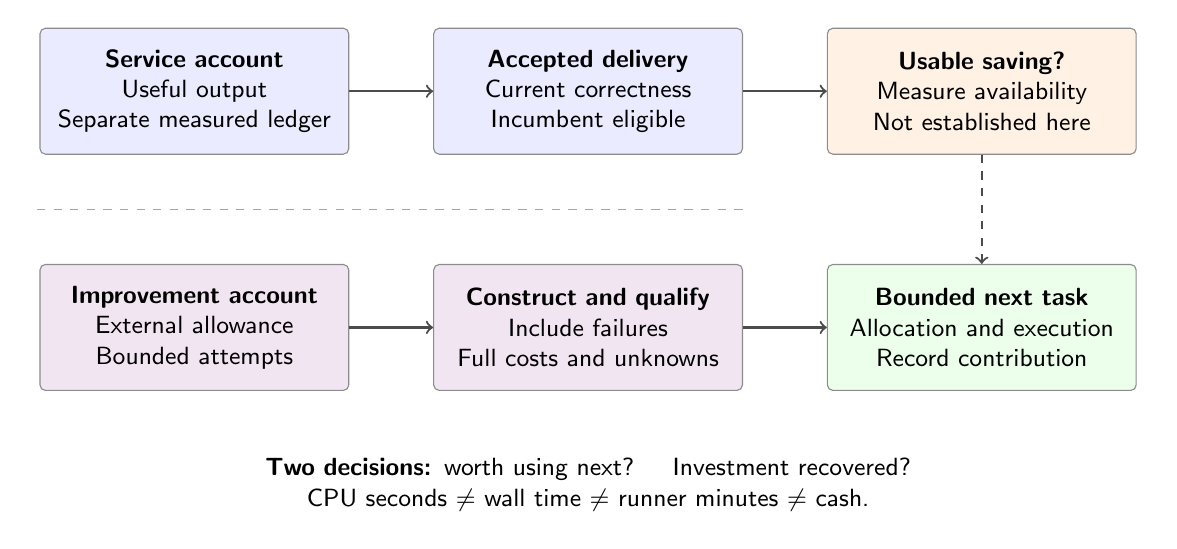
\begin{tikzpicture}[
 font=\sffamily\small,
 box/.style={draw=black!45,rounded corners=2pt,align=center,text width=3.5cm,minimum height=1.6cm,inner sep=6pt},
 flow/.style={->,thick,draw=black!70}]
\node[box,fill=blue!8] (service) at (0,0) {\textbf{Service account}\\Useful output\\Separate measured ledger};
\node[box,fill=blue!8] (delivered) at (5,0) {\textbf{Accepted delivery}\\Current correctness\\Incumbent eligible};
\node[box,fill=orange!10] (available) at (10,0) {\textbf{Usable saving?}\\Measure availability\\Not established here};
\node[box,fill=violet!10] (research) at (0,-3) {\textbf{Improvement account}\\External allowance\\Bounded attempts};
\node[box,fill=violet!10] (build) at (5,-3) {\textbf{Construct and qualify}\\Include failures\\Full costs and unknowns};
\node[box,fill=green!8] (next) at (10,-3) {\textbf{Bounded next task}\\Allocation and execution\\Record contribution};
\draw[flow] (service) -- (delivered);
\draw[flow] (delivered) -- (available);
\draw[flow] (research) -- (build);
\draw[flow] (build) -- (next);
\draw[flow,dashed] (available) -- (next);
\draw[dashed,draw=black!35] (-2,-1.5) -- (7,-1.5);
\node[font=\sffamily\small,align=center,text width=14cm] at (5,-5) {\textbf{Two decisions:} worth using next? \quad Investment recovered?\\CPU seconds $\ne$ wall time $\ne$ runner minutes $\ne$ cash.};
\end{tikzpicture}
\caption{Separate service, investment and feedback accounts. The dashed feedback path requires an actual usable-capacity witness, which this study does not establish. An externally supplied allowance remains external even when the preceding mission was faster. Separate measured accounts do not establish protected operational resource reservation.}
\label{fig:resources}
\end{figure}
